\documentclass[UTF8]{book}
%\documentclass{ctexart}

\usepackage{xeCJK}
%中文支持包

\setCJKmainfont{Microsoft YaHei}  
% 设置默认中文字体是微软雅黑

\setmainfont{Consolas} 
%设置默认的英文字体

\setCJKfamilyfont{kai}{KaiTi}         %定义楷体的字体族代号: kai    
\newcommand{\kai}{\CJKfamily{kai}}    %宏定义kai体命令: \kai{}
%代码中使用: \kai{}  与  \CJKfamily{kai}  是一样的

\setCJKfamilyfont{song}{SimSun}		  %定义宋体的字体族代号: song
\newcommand{\song}{\CJKfamily{song}}  %宏定义song体

\setCJKfamilyfont{Yahei}{Microsoft YaHei}
\newcommand{\Yahei}{\CJKfamily{Yahei}}

%%%%%%%%%%%%%%%%%%%%%%%%%% 以上是字体部分 %%%%%%%%%%%%%%%%%%%%%%%%%%%%%%%

\usepackage{geometry}
\geometry{a4paper, centering , scale=0.8} 			% a4纸, 居中, 占页面80%
%\geometry{left=1cm,right=2cm,top=3cm,bottom=4cm} 	% 页边距



\usepackage{fancyhdr}				 % 页眉页脚
	\pagestyle{fancy}
	\lhead{ }
	\chead{ }
	\rhead{ $L^AT_EX$ }
	\lfoot{}
	\cfoot{\thepage}
	\rfoot{}
	\renewcommand{\headrulewidth}{0pt}           %页眉与正文分割线的粗细
	\renewcommand{\headwidth}{\textwidth}
	\renewcommand{\footrulewidth}{0pt}
%%%%%%%%%%%%%%%%%%%%%%%%%% 以上是页面设置部分 %%%%%%%%%%%%%%%%%%%%%%%%%%%%

\usepackage{listings}    % 插入代码

\lstset{ 
	backgroundcolor=\color{mybackground},   				% choose the background color	
	basicstyle=\footnotesize\color{white},       				% size of fonts used for the code
	numbers=left, 											% 行号加在左边还是有边
	numberstyle=\tiny\color{black},										% 行号的字体设定
	columns=fullflexible,
 	breakatwhitespace=false,         % sets if automatic breaks should only happen at whitespace	
	breaklines=true,                				% automatic line breaking only at whitespace 自动换行
	captionpos=b,                    				% sets the caption-position to bottom
	keepspaces=true,                 % keeps spaces in text, useful for keeping indentation of code (possibly needs columns=flexible)	
	rulecolor=\color{green}, 			
	 showspaces=false,                % show spaces everywhere adding particular underscores; it overrides 'showstringspaces'
	  showstringspaces=false,          % underline spaces within strings only	
	tabsize=4,
	commentstyle=\color{green},   				% comment style
	escapeinside={\%*}{*)},         				% if you want to add LaTeX within your code
	keywordstyle=\color{green},       				% keyword style
	stringstyle=\color{mymauve},     		% string literal style
%	frame=shadowbox,
	frame=single,
	rulesepcolor=\color{red!20!green!20!blue!20},
	% identifierstyle=\color{red},	
	language=[LaTeX]TeX,
	title=\lstname
}

%%%%%%%%%%%%%%%%%%%%%%%%%% 以上是插入代码设置部分 %%%%%%%%%%%%%%%%%%%%%%%%%%

\usepackage{colortbl}
\usepackage{xcolor}

\definecolor{mygreen}{rgb}{0,0.6,0}
\definecolor{mymauve}{rgb}{0.58,0,0.82}
\definecolor{mygray}{gray}{.9}
\definecolor{mypink}{rgb}{.99,.91,.95}
\definecolor{mybackground}{RGB}{45,45,45}

%%%%%%%%%%%%%%%%%%%%%%%%%% 以上是颜色设置部分 %%%%%%%%%%%%%%%%%%%%%%%%%%%

\usepackage{graphicx}   % 插图片
\usepackage{makeidx}   
\usepackage{float}
\usepackage{amsmath}    % 数学公式包
\usepackage{amssymb}
\usepackage{multirow}
\usepackage{booktabs}
\usepackage{setspace}
\usepackage{fontspec}
\usepackage{lipsum}

%%%%%%%%%%%%%%%%%%%%%%%%%% 其余会用到的包 %%%%%%%%%%%%%%%%%%%%%%%%%%%%%%%

% 画图
%\usepackage{tikz}
%\usetikzlibrary{matrix,arrows,shapes,chains}
\usepackage[explicit]{titlesec}
% 衬线字体
%\usepackage{charter}

\definecolor{mybluei}{RGB}{20, 0, 100}
\definecolor{myblueii}{RGB}{0, 0, 100}
\usepackage{rotating, graphicx}

\usepackage{tcolorbox}
\newcommand\ChapterFont{\rmfamily\selectfont\huge}
\newcommand\SectionFont{\bfseries\rmfamily\selectfont\Large}

%chapter
\titleformat{\chapter}[block]
 {\normalfont\ChapterFont\huge\color{myblueii}} 
 {\tcbset{colframe=mybluei, boxrule=0.8pt, left=0pt, right=0pt, top=0pt, bottom=0pt}
  \raisebox{-0.48\height}{\rotatebox{90}{\tcbox[boxsep=4pt, colback= white ]{\color{mybluei}\Large $L^AT_EX$}}}
  \hskip 0.25em
  \mbox{\tcbox[ boxsep=12pt, colback=mybluei, tcbox raise = -35pt]{\color{white}\bfseries\fontsize{70}{70}\selectfont\thechapter}}}
 {0.5em}
 {#1\vskip0.6ex\endgraf\titlerule[1ex]}
 []

%section
 \titleformat{\section}
 {\normalfont\small\sffamily\SectionFont\color{myblueii}}
 {\colorbox{mybluei}{%
        \parbox[c][28pt][c]{40pt}{%
            \centering\textcolor{white}{\SectionFont\Large\rmfamily\thesection}%
        }%
    }%
 }
 {1em}
 {#1}
 [\vspace{-0.755\baselineskip}%
 \color{myblueii}\hspace*{\dimexpr40pt+2\fboxsep\relax}%
 \rule{\dimexpr\textwidth-40pt-2\fboxsep\relax}{1pt}%
 ]
 
% subsection 
 \titleformat{\subsection}
 {\normalfont\small\sffamily\SectionFont\color{myblueii}}
 {\colorbox{mybluei}{%
        \parbox[c][16pt][c]{50pt}{%
            \centering\textcolor{white}{\SectionFont\Large\rmfamily\thesubsection}%
        }%
    }%
 }
 {1em}
 {#1}
 [\vspace{-0.755\baselineskip}%
 \color{myblueii}\hspace*{\dimexpr40pt+2\fboxsep\relax}%
 \rule{\dimexpr\textwidth-40pt-2\fboxsep\relax}{0pt}%
 ]

%%%%%%%%%%%%%%%%%%%%%%%%%% 定制章节头 %%%%%%%%%%%%%%%%%%%%%%%%%%%%%%%



\title{Latex学习手记}
\author{白岩}
\date{\today}

\begin{document}

\tableofcontents
\maketitle

\chapter{第一部分}
\kai{
文档地址: $ http://www.ctex.org/documents/packages/ $

这是我正式决定将我的学习笔记写成电子版的第一篇。\\
纸质版的笔记排版太难受,修改也很麻烦,不如改成电子版的笔记,以后使用起来也很方便。由于写笔记使用的是Latex, 所以第一篇笔记就贡献给Latex了。\\
Latex 是常用的排版工具, 本学习笔记用于自己以后复习和使用查表使用,故有些东西就不用讲的很详细了。\\
Latex 在Windows和Linux上均可以使用, 所以双系统的我就都安装配置了。\\

在此之前,或引用,或自己写,先记录一些基础的入门知识。
}
\vspace*{4em}
\section{简介}
\kai{

	\subsection{Latex家族}
	TeX, pdfTeX, XeTeX, LuaTeX, LaTeX, pdfLaTeX, XeLaTeX …
	\paragraph{Tex}
	{
	 是高德纳(Donald Ervin Knuth,1938年1月10日 –)教授愤世嫉俗(追求完美)做出来的排版引擎,同时也是该引擎使用的标记语言(Markup Lang)的名称。\\
	}
	\paragraph{LaTex} 
	{ 则是 L. Lamport (1941年2月7日 – ) 教授开发的基于 TeX 的排版系统。实际上 LaTeX 利用 TeX 的控制命令,定义了许多新的控制命令并封装成一个可执行文件。这个可执行文件会去解释 LaTeX 新定义的命令成为 TeX 的控制命令,并最终交由 TeX 引擎进行排版。\\
	}\\
	因此在 TeX - LaTeX 组合中,\\
	最终进行断行、分页等操作的,是 TeX 引擎;\\
	LaTeX 实际上是一个工具,它将用户按照它的格式编写的文档解释成 TeX 引擎能理解的形式并交付给 TeX 引擎处理,再将最终结果返回给用户。\\
	\paragraph{pdfTex - pdfLaTex}
	{
	TeX 系统生成的文件是 dvi 格式,虽然可以用其他程序将其转换为例如 pdf 等更为常见的格式,但是毕竟不方便。
	为了解决这个问题,Hàn Thế Thành 博士在他的博士论文中提出了 pdfTeX 这个对 TeX 引擎的扩展。二者最主要的差别就是 pdfTeX 直接输出 pdf 格式文档,而 TeX 引擎则输出 dvi 格式的文档。\\
	pdfLaTeX 这个程序的主要工作依旧是将 LaTeX 格式的文档进行解释,不过此次是将解释之后的结果交付给 pdfTeX 引擎处理。
	}
	\paragraph{XeTeX - XeLaTeX}
	{
	高德纳教授在实现 TeX 的当初并没有考虑到中日韩等字符的处理,而只支持 ASCII 字符。这并不是说中日韩字符就无法使用 TeX 引擎排版了,事实上 TeX 将每个字符用一个框包括起来(这被称为盒子)然后将一个个的盒子按照一定规则排列起来,因而 TeX 的算法理论上适用于任何字符。ASCII 字符简单理解,就是在半角模式下你的键盘能直接输出的字符。

在 XeTeX 出现之前,为了能让 TeX 系统排版中文,国人曾使用了 天元、CCT、CJK 等手段处理中文。其中 天元和CCT 现在已经基本不用,CJK 因为使用时间长且效果相对较好,现在还有人使用。

不同于 CJK 等方式使用 TeX 和 pdfTeX 这两个不直接支持 Unicode 字符的引擎,XeTeX 引擎直接支持 Unicode 字符。也就是说现在不使用 CJK 也能排版中日韩文的文档了,并且这种方式要比之前的方式更加优秀。

XeLaTeX 和 XeTeX 的关系与 pdfLaTeX 和 pdfTeX 的关系类似,这里不再赘述。

使用 XeTeX 引擎需要使用 UTF-8 编码。

所谓编码就是字符在计算机储存时候的对应关系。例如,假设有一种编码,将汉字「你」对应为数字「1」;「好」对应为数字「2」,则含有「你好」的纯文本文件,在计算机中储存为「12」(读取文件的时候,将「12」再转换为「你好」显示在屏幕上或打印出来)。

UTF-8 编码是 Unicode 编码的一种.
	}
	
	\subsection{发行版}
	CTeX, MiKTeX, TeX Live 都是被称为「发行」的软件合集。他们包括了上述各种引擎的可执行程序,以及一些文档类、模板、字体文件、辅助程序等等。其中 CTeX 是建立在 MiKTeX 的基础之上的。
	
	TexLive 是跨平台可使用的。故我使用的主要就是TexLive。
}
\vspace*{4em}
\section{安装与配置}
\kai{
\subsection{Windows}
Windows下的安装是很简单的。 \\
一般我不使用Texwork作为编辑环境,我使用Texmaker作为写LaTex文档的编辑器。\\
TexLive 和 Texmaker 的安装顺序没有要求。\\

	{\Large{<TexLive>}}
	
下载Texlive的镜像文件,大概3GB左右。 然后双击安装就可以了。记住安装的文件夹,在安装的时候有些功能可以选择安装或不安装。比如Texwork就不用安装了。\\

	{\Large{<Texmaker>}}

这个的安装也是十分的简单, 首先下载软件,然后双击安装就好了。\\

	{\Large{<配置Texmaker>}}
	
打开Texmaker, 找到 "选项" -> "配置Texmaker"。 命令栏修改参数如图:\\
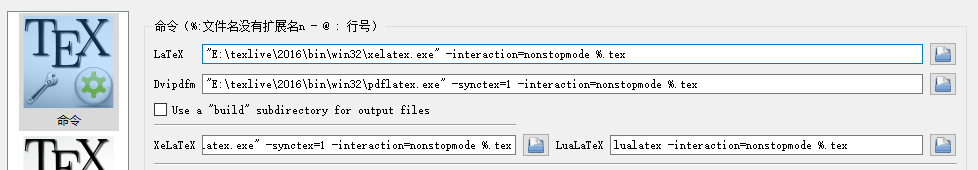
\includegraphics[width=6.0in]{1.png}\\
其中双引号中的路径是你的TexLive安装的路径,对应相应的可执行文件。需要修改的位置有三处, 除了上面两处还有xeLaTex,内容与Latex一致。\\
可以发现,这里我们使用的都是xeLatex 来进行编译解析。

下面配置 "快速启动" 选项。\\
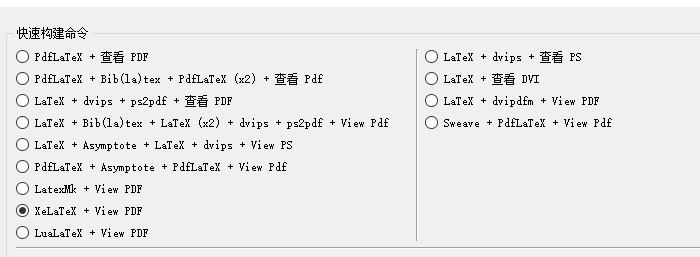
\includegraphics[width=6.0in]{2.png}\\
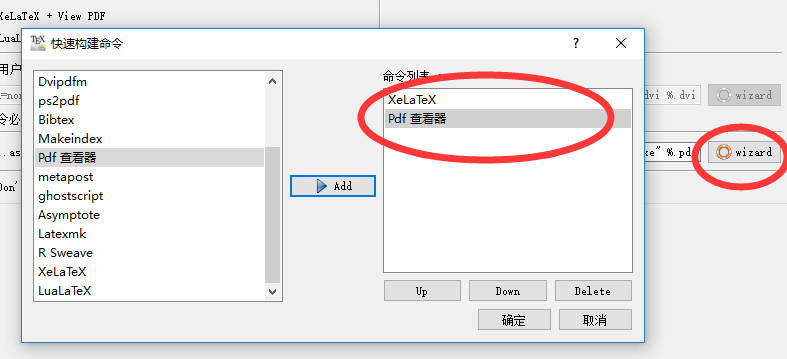
\includegraphics[width=6.0in]{3.png}\\
快速启动需要配置快速启动的组合,和相应的处理程序。如上图,不多说。

\subsection{Linux-Ubuntu}
Linux 下的安装也是比较简单的。

首先使用命令安装
 \begin{lstlisting}
	sudo apt-get install texlive-latex-base 
	sudo apt-get install latex-cjk-all 
	sudo apt-get install texmaker
 \end{lstlisting}

 这样基本的就安装完毕了,如果在运行的过程中会有写文件找不到,在错误的信息里可以看到 缺少.sty, 此时就用命令查一下, 然后安装就行了。命令如下:
  \begin{lstlisting}
	apt-cache search lastpage (注意不要加.sty文件后缀)

	// 可以看到需要下面的包,以及对这个包的描述:
	texlive-latex-extra - TeX Live: LaTeX supplementary packages

	// 选择安装即可:
	sudo apt-get install texlive-latex-extra

 \end{lstlisting}
	
	{\Large{<配置Texmaker>}}
	
	配置的过程几乎是一样的,不同的就是在这里的xelatex 选项不需要配置到相应的文件夹了。
	将Latex选项配置为xeLatex命令就可以了。
	其余的不变。	
	
	此外关于字体, 可以使用命令查看现有的系统的字体: `fc-list :lang=zh-cn`
}
\vspace*{4em}
\section{基本设置}
\kai{
这里记录一下导言区常用的包的配置等等。

 \begin{lstlisting}
 常用的导言区会在本文档的源文件中。
 \end{lstlisting}
 
 1. 常用的文档类型有: article、report、book 等。其中article从Section开始, report从chapter开始, Book从part开始。
 
 2. 除了使用CJK包来实现中英文混排,还可以直接使用cTex来实现。使用cTex只需要在documentclass的时候指定[UTF8]\{ctexart\}\{ctexrep\}\{ctexbook\}

 3. 部分中带星号的属于不进行编号的部分。 
 }
\vspace*{4em}
\section{newcommand 自定义命令}
{\kai{
使用$newcommand$可以自己定制命令\\
语法格式:\\
\begin{lstlisting}

	\ newcommand{\yourcommand}[参数个数]{内容}

比如:
	\ newcommand{\wuhao}{\fontsize{10.5pt}{10.5pt}\selectfont}

% 说明 \fontsize{}{}与\selectfont是LaTeX提供的字号控制低级命令,供用户自己设置字号大小。
% \fontsize{参数1}{参数1}中参数1为字号大小,参数2为行间距,
% 只有使用\selectfont命令之后,\fontzize{}{}的设置才能生效。切记
\end{lstlisting}
}}
\vspace*{4em}
\section{版面设置}
\kai{
	\subsection{页面设置}
	这部分直接参见源文件中的设置就可以了, 可以设置纸张的大小,各个边的页边距等。
	
	\subsection{页眉页脚}
	使用到的宏包是: fancyhdr
	
	在页眉左边写上我的名字,中间写上今天的日期,右边写上我的电话;页脚的正中写上页码;页眉和正文之间有一道宽为 0.4pt 的横线分割,可以在导言区加上如下几行:
	\begin{lstlisting}
	\usepackage{fancyhdr}
	\pagestyle{fancy}
	\lhead{\author}
	\chead{\date}
	\rhead{152xxxxxxxx}
	\lfoot{}
	\cfoot{\thepage}
	\rfoot{}
	\renewcommand{\headrulewidth}{0.4pt}
	\renewcommand{\headwidth}{\textwidth}
	\renewcommand{\footrulewidth}{0pt}
	\end{lstlisting}
	
	\subsection{首行缩进}
	CTex 已经处理了首行缩进的问题,使用xeCJK需要用下面的方法。
	\begin{lstlisting}

	\usepackage{indentfirst}
	//就算是这样,首行缩进的长度,仍然不符合中国人的习惯。我们可以在导言区添加这样的控制序列 
	\setlength{\parindent}{\ccwd} 
	// 来调整首行缩进的大小。这里的 \ccwd 是当前字号下一个中文汉字的宽度。

	\end{lstlisting}
	
	\subsection{行间距}
	\begin{lstlisting}
	
	\usepackage{setspace}
	\onehalfspacing

	\end{lstlisting}
	
	\subsection{段间距}
	\begin{lstlisting}
	
	\addtolength{\parskip}{.4em}
	// 相对于原来的加0.4  如果要减小就填负数。
	
	\end{lstlisting}
	
The space between paragraphs, sections, subsections, etc. is determined automatically by LaTeX. If you want to customize the default paragraph spacing, it can be achieved with the following command in the preamble of your document:
\begin{lstlisting}
\parskip 7.2pt
\end{lstlisting}
Additional space between two lines of the same paragraph or within a table is specified with the
\begin{lstlisting}
 \\[length] 
\end{lstlisting}
If you want to add space at the beginning of the document, without anything else written before, then you may use
\begin{lstlisting}
{ \vspace*{length} } 
\end{lstlisting}
}
\vspace*{4em}
\section{表格}
\kai{
 1. 第一种最普通的表格形式\\
 
 \begin{lstlisting}
	\begin{tabular}{|l|c|r|}
	 \hline
	操作系统& 发行版& 编辑器\\
	 \hline
	Windows & MikTeX & TexMakerX \\
	 \hline
	Unix/Linux & teTeX & Kile \\
	 \hline
	Mac OS & MacTeX & TeXShop \\
	 \hline
	通用& TeX Live & TeXworks \\
	 \hline
	\end{tabular}
	
	\begin{tabular}{ p{7em} p{23em} }  % 用于指定列的宽度。
	\caption{示例表格}                   % 用于给表格加标题。 
 \end{lstlisting}
* 其中\{|l|c|r|\}分别指定每一列的对齐方式。竖线代表竖格线,没有就代表没有格线\\
* hline 代表横格线\\
* \& 用于列分隔\\

	\begin{tabular}{|l|c|r|}
	 \hline
	操作系统& 发行版& 编辑器\\
	 \hline
	Windows & MikTeX & TexMakerX \\
	 \hline
	Unix/Linux & teTeX & Kile \\
	 \hline
	Mac OS & MacTeX & TeXShop \\
	 \hline
	通用& TeX Live & TeXworks \\
	 \hline
	\end{tabular}\\
	
	2. 交替明暗的表格。三线式表格,可以指定每一个格子的颜色。\\
	
	\begin{lstlisting}
	\begin{tabular}{>{\sf }lll}    %
	\toprule	
	标签 & 描述 \\
	\midrule
	<b>	& \kai 定义粗体文本\\
	\rowcolor{mygray}          % 下一行的颜色
	<em> & \kai 定义着重文字\\
	<i> & \kai 定义斜体文字\\
	\rowcolor{mygray}
	<small> & \kai 定义小号文字\\
	<strong> & \kai 定义大号文字\\
	\rowcolor{mygray}
	<sub> & \kai 定义下标 \\
	<sup> & \kai 定义上标 \\
	\rowcolor{mygray}
	\bottomrule
	\end{tabular}
	\end{lstlisting}
	
	\begin{tabular}{>{\sf }lll}    %
	\toprule	
	标签 & 描述 \\
	\midrule
	<b>	& \kai 定义粗体文本\\
	\rowcolor{mygray}          % 下一行的颜色
	<em> & \kai 定义着重文字\\
	<i> & \kai 定义斜体文字\\
	\rowcolor{mygray}
	<small> & \kai 定义小号文字\\
	<strong> & \kai 定义大号文字\\
	\rowcolor{mygray}
	<sub> & \kai 定义下标 \\
	<sup> & \kai 定义上标 \\
	\rowcolor{mygray}
	\bottomrule
	\end{tabular}\\
	
	3. 为列指定颜色。
	\begin{lstlisting}
	\begin{tabular}{>{\columncolor{mypink}\sf }lll@{}}
	\toprule
	\rowcolor{white}
		 & \multicolumn{2}{c}{\bf Specific Heats} \\
		\cmidrule{2-3}
	\rowcolor{white}
		 & $c$ (J/kg$\cdot$K) & $C$ (J/mol$\cdot$K) \\
	\midrule
	Aluminum     & 900  & 24.3 \\
	Copper       & 385  & 24.4 \\
	Gold         & 130  & 25.6 \\
	Steel/Iron   & 450  & 25.0 \\
	\bottomrule
	\end{tabular}
	\end{lstlisting}
	
	\begin{tabular}{>{\columncolor{mypink}\sf }lll@{}}
	\toprule
	\rowcolor{white}
		 & \multicolumn{2}{c}{\bf Specific Heats} \\
		\cmidrule{2-3}
	\rowcolor{white}
		 & $c$ (J/kg$\cdot$K) & $C$ (J/mol$\cdot$K) \\
	\midrule
	Aluminum     & 900  & 24.3 \\
	Copper       & 385  & 24.4 \\
	Gold         & 130  & 25.6 \\
	Steel/Iron   & 450  & 25.0 \\
	\bottomrule
	\end{tabular}\\
	

\colorbox{mypink}{
	\begin{tabular}{@{}>{\sf }lll@{}}
	\toprule
	 & \multicolumn{2}{c}{\bf Specific Heats} \\
	\cmidrule{2-3}
	 & $c$ (J/kg$\cdot$K) & $C$ (J/mol$\cdot$K) \\
	\midrule
	Aluminum     & 900  & 24.3 \\
	Copper       & 385  & 24.4 \\
	Gold         & 130  & 25.6 \\
	Steel/Iron   & 450  & 25.0 \\
	Lead         & 130  & 26.8 \\
	Water        & 4190 & 75.4 \\
	Ice ($-$10 \textcelsius) & 2100 & 38 \\
	\bottomrule
	\end{tabular}
}

\begin{tabular}{|l|
>{\columncolor{yellow}}c|c|>{\columncolor{yellow}}c|c|
>{\columncolor{red}\bfseries}c<{\textsc{GBP}}|}
\hline
\multicolumn{3}{>{\columncolor{red}}l}{\color{white}\textsf{LONDON}}
&\multicolumn{3}{>{\columncolor{red}}r}{\color{white}\textsf{Price}}
\\[1pt]
\hline

Sydney & OG4G &Thu Oct 10 &Mon Oct 21 or 28 &11 or 18 days &999\\

& &Thu Oct 17 &Mon Oct 21 or 28 & 4 or 11 days &999\\

& OG7A &Sun Oct 13 &Mon Oct 21 or 28 & 8 or 15 days &999\\

& &Sun Oct 20 &Mon Oct 28 & 8 days &999\\

\hline

\end{tabular}

其他的表格可以参照2016Penta.tex  
}
\vspace*{4em}
\section{数学公式}
\kai{
数学公式有行内公式和独立公式两种;
\begin{lstlisting}

行内公式就直接使用两个美元符号夹起来就好啦: $ ... $

独立公式使用 \[ ... \] 

若要对公式进行编号就使用
	\begin{equation}
	...
	\end{equation}

\end{lstlisting}

	\subsection{根式 \& 分式 }
	\begin{lstlisting}
	根式	\sqrt{}
	分式 \frac{}{}
	\end{lstlisting}
	\subsection{定界符}
	\begin{lstlisting}
	// 小括号
	\[ \Biggl(\biggl(\Bigl(\bigl((x)\bigr)\Bigr)\biggr)\Biggr) \]
	
	//中括号
	\[ \Biggl[\biggl[\Bigl[\bigl[[x]\bigr]\Bigr]\biggr]\Biggr] \]

	// 大括号
	\[ \Biggl \{\biggl \{\Bigl \{\bigl \{\{x\}\bigr \}\Bigr \}\biggr \}\Biggr\} \]

	// 尖括号
	\[ \Biggl\langle\biggl\langle\Bigl\langle\bigl\langle\langle x
	\rangle\bigr\rangle\Bigr\rangle\biggr\rangle\Biggr\rangle \]	

	\[ \Biggl\lvert\biggl\lvert\Bigl\lvert\bigl\lvert\lvert x
	\rvert\bigr\rvert\Bigr\rvert\biggr\rvert\Biggr\rvert \]	

	\[ \Biggl\lVert\biggl\lVert\Bigl\lVert\bigl\lVert\lVert x
	\rVert\bigr\rVert\Bigr\rVert\biggr\rVert\Biggr\rVert \]

	\end{lstlisting}
	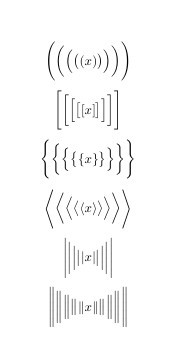
\includegraphics[width=1.5in]{4.jpg}
	
	\subsection{省略号}
	\begin{lstlisting}
	
	// 横版省略号 
	\[ x_1,x_2,\dots ,x_n\quad 1,2,\cdots ,n\quad
	
	// 竖版省略号
	\vdots\quad \ddots \]

	% 对应的 \cdot 是点乘, \dot 是在符号上方加点。
	\end{lstlisting}
	\[ x_1,x_2,\dots ,x_n\quad 1,2,\cdots ,n\quad \vdots\quad \ddots \]
	
	\subsection{连续求和 \& 求积}

	\begin{lstlisting}
		\sum_{i=1}^{n}

		%如果是行内公式,这样的上下标是在右侧的,如果是独立公式,是在上下的。
		%如果要改变位置,可以使用 \sum\limits_{}^{}  和 \sum\nolimits_{}^{}
		% 前者用于行内公式,后者用于独立公式。
	\end{lstlisting}

	\subsection{矩阵}
	\begin{lstlisting}
	
	\[ \begin{pmatrix} a&b\\c&d \end{pmatrix} \quad
	
	\begin{bmatrix} a&b\\c&d \end{bmatrix} \quad
	
	\begin{Bmatrix} a&b\\c&d \end{Bmatrix} \quad
	
	\begin{vmatrix} a&b\\c&d \end{vmatrix} \quad
	
	\begin{Vmatrix} a&b\\c&d \end{Vmatrix} \]

	\end{lstlisting}
	\[ \begin{pmatrix} a&b\\c&d \end{pmatrix} \quad
	\begin{bmatrix} a&b\\c&d \end{bmatrix} \quad
	\begin{Bmatrix} a&b\\c&d \end{Bmatrix} \quad
	\begin{vmatrix} a&b\\c&d \end{vmatrix} \quad
	\begin{Vmatrix} a&b\\c&d \end{Vmatrix} \]
	
	\subsection{多行公式}
	\begin{lstlisting}
	// 公式对齐版本
	\[\begin{aligned}
	x ={}& a+b+c+{} \\
	&d+e+f+g
	\end{aligned}\]
	\end{lstlisting}
		\[\begin{aligned}
	x ={}& a+b+c+{} \\
	&d+e+f+g
	\end{aligned}\]
	
	\subsection{公式组}
	\begin{lstlisting}
	// 公式对齐版本
	\begin{gather}
	a = b+c+d \\
	x = y+z
	\end{gather}	
	\begin{align}	
	a &= b+c+d \\	
	x &= y+z
	\end{align}
	\end{lstlisting}
	
	\begin{gather}
	a = b+c+d \\
	x = y+z
	\end{gather}	
	\begin{align}	
	a &= b+c+d \\	
	x &= y+z
	\end{align}
	
	\subsection{分段函数}
	\begin{lstlisting}
	
	// 用Cases来实现分段
	\[ y= \begin{cases}
	-x,\quad x\leq 0 \\
	x,\quad x>0
	\end{cases} \]

	\end{lstlisting}
	\[ y= \begin{cases}
	-x,\quad x\leq 0 \\
	x,\quad x>0
	\end{cases} \]

}
\vspace*{4em}
\section{代码排版}
{\kai{
排版代码主要使用的包是: listings

If you just want to write code within your document the package provides the lstlisting environment:
\begin{lstlisting}

	\begin{lstlisting}
	Put your code here.
	\ end{lstlisting}

\end{lstlisting}

Another possibility, that is very useful if you created a program on several files and you are still editing it, is to import the code from the source itself. This way, if you modify the source, you just have to recompile the LaTeX code and your document will be updated. The command is:
\begin{lstlisting}

	\lstinputlisting{source_filename.py}

	\lstinputlisting[language=Python]{source_filename.py}
	
	\lstinputlisting[language=Python, firstline=37, lastline=45]{source_filename.py}
	
\end{lstlisting}

	\paragraph{Support Language}

It supports the following programming languages:

\noindent ABAP, ACSL, Ada, Algol, Ant, Assembler, Awk, bash, Basic, C\#, C++, C, Caml, Clean, Cobol, Comal, csh, Delphi, Eiffel, Elan, erlang, Euphoria, Fortran, GCL, Gnuplot, Haskell, HTML, IDL, inform, Java, JVMIS, ksh, Lisp, Logo, Lua, make, Mathematica, Matlab, Mercury, MetaPost, Miranda, Mizar, ML, Modelica, Modula-2, MuPAD, NASTRAN, Oberon-2, Objective C , OCL, Octave, Oz, Pascal, Perl, PHP, PL/I, Plasm, POV, Prolog, Promela, Python, R, Reduce, Rexx, RSL, Ruby, S, SAS, Scilab, sh, SHELXL, Simula, SQL, tcl, TeX, VBScript, Verilog, VHDL, VRML, XML, XSLT.

	\paragraph{Settings}	
一些设置参数。

\begin{lstlisting}

  backgroundcolor=\color{white},   % choose the background color; you must add \usepackage{color} or \usepackage{xcolor}; should come as last argument
  basicstyle=\footnotesize,        % the size of the fonts that are used for the code
  breakatwhitespace=false,         % sets if automatic breaks should only happen at whitespace
  breaklines=true,                 % sets automatic line breaking
  captionpos=b,                    % sets the caption-position to bottom
  commentstyle=\color{mygreen},    % comment style
  deletekeywords={...},            % if you want to delete keywords from the given language
  extendedchars=true,              % lets you use non-ASCII characters; for 8-bits encodings only, does not work with UTF-8
  frame=single,	                   % adds a frame around the code
  keepspaces=true,                 % keeps spaces in text, useful for keeping indentation of code (possibly needs 				columns=flexible)
  keywordstyle=\color{blue},       % keyword style
  language=Octave,                 % the language of the code
  morekeywords={*,...},           % if you want to add more keywords to the set
  numbers=left,                    % where to put the line-numbers; possible values are (none, left, right)
  numbersep=5pt,                   % how far the line-numbers are from the code
  numberstyle=\tiny\color{mygray}, % the style that is used for the line-numbers
  rulecolor=\color{black},         % if not set, the frame-color may be changed on line-breaks within not-black text (e.g. comments (green here))
  showspaces=false,                % show spaces everywhere adding particular underscores; it overrides 'showstringspaces'
  showstringspaces=false,          % underline spaces within strings only
  showtabs=false,                  % show tabs within strings adding particular underscores
  stepnumber=2,                    % the step between two line-numbers. If it's 1, each line will be numbered
  stringstyle=\color{mymauve},     % string literal style
  tabsize=2,	                   % sets default tabsize to 2 spaces
  title=\lstname                   % show the filename of files included with \lstinputlisting; also try caption instead of title
        
\end{lstlisting}

更多详细信息查看:$ https://en.wikibooks.org/wiki/LaTeX/Source_Code_Listings$

文档:$ http://mirror.lzu.edu.cn/CTAN/macros/latex/contrib/listings/listings.pdf$
}}
\vspace*{4em}
\section{定制章节样式}
\kai{
使用titlesec包来定制属于自己的样式。

\begin{lstlisting}

\usepackage[explicit]{titlesec}

\definecolor{mybluei}{RGB}{20, 0, 100}
\definecolor{myblueii}{RGB}{0, 0, 100}
\usepackage{rotating, graphicx}

\usepackage{tcolorbox}
\newcommand\ChapterFont{\rmfamily\selectfont\huge}
\newcommand\SectionFont{\bfseries\rmfamily\selectfont\Large}

%chapter
\titleformat{\chapter}[block]
 {\normalfont\ChapterFont\huge\color{myblueii}} 
 {\tcbset{colframe=mybluei, boxrule=0.8pt, left=0pt, right=0pt, top=0pt, bottom=0pt}
  \raisebox{-0.48\height}{\rotatebox{90}{\tcbox[boxsep=4pt, colback= white ]{\color{mybluei}\Large $L^AT_EX$}}}
  \hskip 0.25em
  \mbox{\tcbox[ boxsep=12pt, colback=mybluei, tcbox raise = -35pt]{\color{white}\bfseries\fontsize{70}{70}\selectfont\thechapter}}}
 {0.5em}
 {#1\vskip0.6ex\endgraf\titlerule[1ex]}
 []

%section
 \titleformat{\section}
 {\normalfont\small\sffamily\SectionFont\color{myblueii}}
 {\colorbox{mybluei}{%
        \parbox[c][28pt][c]{40pt}{%
            \centering\textcolor{white}{\SectionFont\Large\rmfamily\thesection}%
        }%
    }%
 }
 {1em}
 {#1}
 [\vspace{-0.755\baselineskip}%
 \color{myblueii}\hspace*{\dimexpr40pt+2\fboxsep\relax}%
 \rule{\dimexpr\textwidth-40pt-2\fboxsep\relax}{1pt}%
 ]
 
% subsection 
 \titleformat{\subsection}
 {\normalfont\small\sffamily\SectionFont\color{myblueii}}
 {\colorbox{mybluei}{%
        \parbox[c][16pt][c]{50pt}{%
            \centering\textcolor{white}{\SectionFont\Large\rmfamily\thesubsection}%
        }%
    }%
 }
 {1em}
 {#1}
 [\vspace{-0.755\baselineskip}%
 \color{myblueii}\hspace*{\dimexpr40pt+2\fboxsep\relax}%
 \rule{\dimexpr\textwidth-40pt-2\fboxsep\relax}{0pt}%
 ]


具体的用法事实上我也不是很清楚。从上面的代码中我们可以窥探一些用法。
\end{lstlisting}

具体的用法事实上我也不是很清楚。从上面的代码中我们可以窥探一些用法。

colorbox 这个是用来画一个颜色块。颜色块内可以放文字或表格。之前在做表格的时候我们使用过这个元素。\\
基本语法:
\begin{lstlisting}
\colorbox{\color{blue}} {Text}
\end{lstlisting}
两个参数,分别是颜色、内容。

在使用这里的内容的时候我们也可以窥探一些其他东西。这里就是Latx中很重要的盒子。

	\subsection{盒子}
所谓盒子就是一部分文本,tex把它当作一个整体,如同单个字符一样处理!

实际上,tex内部格式化的方式也是如此,单个字符构成一个盒子,然后把它放到水平的行盒子里面,在单词间插入橡皮长度。行盒子竖直堆积,构成段落盒子,在行之间也要插入橡皮长度,然后把它们放到页面主体盒子中,连同页眉和页脚盒子构成页面盒子!

在latex里面有三种类型的盒子,LR盒子,段落盒子,标尺盒子。
\begin{itemize}
\item LR盒子是由水平的从左到右的有序材料组成。
\item 段落盒子是竖直堆积的行组成。
\item 标尺盒子是一个用黑色填充的实心矩形。通常用来画水平或竖直线!
\end{itemize}

LR盒子:
\begin{lstlisting}
\mbox{文本} 和 \makebox[宽度][位置]{文本}
\fbox{文本} 和 \framebox[宽度][位置]{文本}
\end{lstlisting}

左边两条命令生成一个LR盒子,其宽度恰好是在\{ \}中给出的文本的宽度! fbox 有外框!

右面命令宽度是由可省的长度参数来预先确定的,另一个可省参数位置定义文本在盒子的位置,如果不给出的,文本时居中排列的,位置参数可以取如下值:l  r  s  

文本的自然宽度要比所定义的宽度大的时候,就会出现突出! 

makebox命令很有用,可在picture环境中生成一个居中的或者左右对齐的文本,也可以使部分文本重叠!如 makebox[0pt][1]\{/\}S,结果是一条斜线穿过S。长度定义必须含有单位。
\begin{lstlisting}
\newsavebox{\boxname}
\end{lstlisting}
初始化之后,使用命令 
\begin{lstlisting}
\sbox{\boxname}{文本}或者 \savebox[宽度][位置]{文本}
\end{lstlisting}
就会把文本的内容保存起来以备后用。使用时
\begin{lstlisting}
\usebox{\boxname} 插入保存的文本。
\end{lstlisting}

LR盒子的内容也可以用如下环境保存
\begin{lstlisting}
\begin{lrbox}{boxname}   文本  \end{lrbox}
\end{lstlisting}

LR盒子的竖直移位
\begin{lstlisting}
\raisebox{上移量}[高度][深度]{文本}
\end{lstlisting}

子段盒子和小页:

生成给定宽度的盒子,其中的文本行如通常的段落模式一样彼此堆积,命令如下
\begin{lstlisting}
\parbox[位置]{宽度}{文本}或者 \begin{minipage}[位置]{宽度} 文本\end{minipage}
\end{lstlisting}
可省参数位置可取值: b t, 默认是居中排列。

竖直摆放的问题,对齐两个小页,需要加入 mbox的空行\\
具有指定高度的段落盒子\\
命令是tex命令的扩展。

标尺盒子:
\begin{lstlisting}
\rule[提示]{宽度}{高度}
\end{lstlisting}
也可以生成一个宽度为零的标尺盒子,这样得到一个不可见的具有给定高度的盒子,如此的构造称为一个支撑,如此可以强迫所在的水平盒子具有不同于其所包含内容需要的高度和深度!

嵌套盒子:

盒子的样式参数,对于有框盒子 fboxrule 确定方框线的粗细  fboxsep  设置方框与被包围文本之间的距离大小。

}
\kai{

}

\end{document}
